\documentclass[a4paper,12pt,twoside]{memoir}


% Castellano
\usepackage[spanish,es-tabla]{babel}
\selectlanguage{spanish}
\usepackage[utf8]{inputenc}
\usepackage[T1]{fontenc}
\usepackage{lmodern} % scalable font
\usepackage{microtype}
\usepackage{placeins}

\RequirePackage{booktabs}
\RequirePackage[table]{xcolor}
\RequirePackage{xtab}
\RequirePackage{multirow}

% Links
\PassOptionsToPackage{hyphens}{url}\usepackage[colorlinks]{hyperref}
\hypersetup{
	allcolors = {red}
}

% Ecuaciones
\usepackage{amsmath}

% Rutas de fichero / paquete
\newcommand{\ruta}[1]{{\sffamily #1}}

% Párrafos
\nonzeroparskip

% Huérfanas y viudas
\widowpenalty100000
\clubpenalty100000

% Evitar solapes en el header
\nouppercaseheads


\let\tmp\oddsidemargin
\let\oddsidemargin\evensidemargin
\let\evensidemargin\tmp
\reversemarginpar



% Imagenes
\usepackage{graphicx}
\newcommand{\imagen}[2]{
	\begin{figure}[!h]
		\centering
		\includegraphics[width=0.9\textwidth]{#1}
		\caption{#2}\label{fig:#1}
	\end{figure}
	\FloatBarrier
}






\graphicspath{ {./img/} }

% Capítulos
\chapterstyle{bianchi}
\newcommand{\capitulo}[2]{
	\setcounter{chapter}{#1}
	\setcounter{section}{0}
	\setcounter{figure}{0}
	\setcounter{table}{0}
	\chapter*{#2}
	\addcontentsline{toc}{chapter}{#2}
	\markboth{#2}{#2}
}

% Apéndices
\renewcommand{\appendixname}{Apéndice}
\renewcommand*\cftappendixname{\appendixname}

\newcommand{\apendice}[1]{
	%\renewcommand{\thechapter}{A}
	\chapter{#1}
}

\renewcommand*\cftappendixname{\appendixname\ }

% Formato de portada
\makeatletter
\usepackage{xcolor}
\newcommand{\tutor}[1]{\def\@tutor{#1}}
%\newcommand{\tutorb}[1]{\def\@tutorb{#1}}
\newcommand{\course}[1]{\def\@course{#1}}
\definecolor{cpardoBox}{HTML}{E6E6FF}
\def\maketitle{
  \null
  \thispagestyle{empty}
  % Cabecera ----------------
\begin{center}
  \noindent
\includegraphics[width=\textwidth]{cabeceraSalud}\vspace{1.5cm}%
\end{center}

  
  % Título proyecto y escudo salud ----------------

  \begin{center}
    \begin{minipage}[c][1.5cm][c]{.20\textwidth}
        
\includegraphics[width=\textwidth]{escudoSalud.pdf}
    \end{minipage}
  \end{center}
  
  \begin{center}
    \colorbox{cpardoBox}{%
        \begin{minipage}{.8\textwidth}
          \vspace{.5cm}\Large
          \begin{center}
          \textbf{TFG del Grado en Ingeniería de la Salud}\vspace{.6cm}\\
          \textbf{\LARGE\@title{}}
          \end{center}
          \vspace{.2cm}
        \end{minipage}
    }%
  \end{center}
  
    % Datos de alumno, curso y tutores ------------------
  \begin{center}%
  {%
    \noindent\LARGE
    Presentado por \@author{}\\ 
    en Universidad de Burgos\\
    \vspace{0.5cm}
    \noindent\Large
    \@date{}\\
    \vspace{0.5cm}
    Tutor: \@tutor{}\\ % comenta el que no corresponda
    %Tutores: \@tutor{} -- \@tutorb{}\\
  }%
  \end{center}%
  \null
  \cleardoublepage
  }
\makeatother



% Datos de portada
\title{Detección de la actividad muscular de las personas con Párkinson \\Documentación Técnica}
\author{Sara Ruishan González Bárcena}
\tutor{Guirguis Zaki Guirguis Abdelmessih}
%\tutorb{nombre tutor 2}
\date{\today}

\begin{document}

\maketitle



\cleardoublepage



%%%%%%%%%%%%%%%%%%%%%%%%%%%%%%%%%%%%%%%%%%%%%%%%%%%%%%%%%%%%%%%%%%%%%%%%%%%%%%%%%%%%%%%%



\frontmatter


\clearpage

% Indices
\tableofcontents

\clearpage

\listoffigures

\clearpage

\listoftables

\clearpage

\mainmatter

\appendix



\apendice{Plan de Proyecto Software}

\section{Introducción}

%Ojo \footnote{Los anexos deben de tener su propia bibliografía, eso es tan fácil como utilizar referencias igual que en la memoria \cite{bortolot2005}}

\section{Planificación temporal}

\begin{figure}[ht]
    \centering
    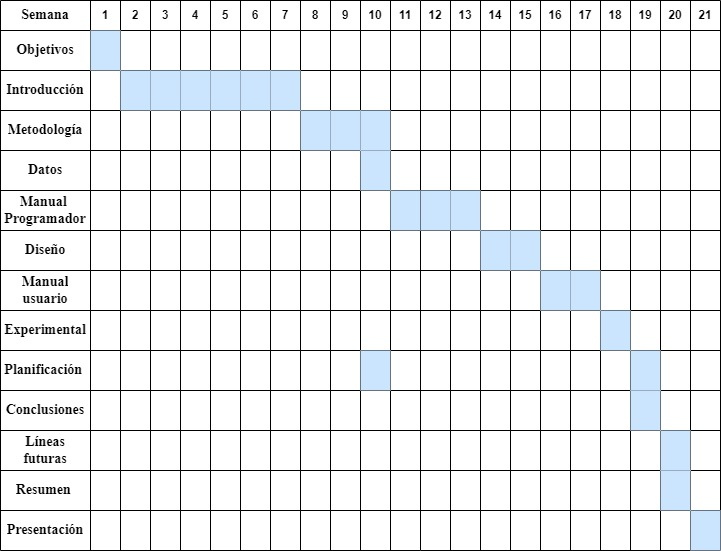
\includegraphics[width=0.85\textwidth]{img/planificacionTFG.jpg}
    \caption{Planificación temporal}
    \label{fig:plan-temporal}
 \end{figure}

\subsection{Planificación económica}

\begin{table}[ht]
	\centering
	\begin{tabularx}{\linewidth}{ p{0.6\columnwidth} p{0.71\columnwidth} }
		\toprule
		\textbf{Materiales}    & \textbf{Precio}\\
		\toprule
		\textbf{Placa Arduino Uno}              & precio \\
		\textbf{MPU-6050}                & precio \\
        \textbf{Módulo HC-05}              & precio    \\
        \textbf{Módulo ESP8266}              & precio    \\
		\bottomrule
	\end{tabularx}
	\caption{Planificación económica}
\end{table}

\subsection{Viabilidad legal}


\apendice{Documentación de usuario}

\section{Requisitos software y hardware para ejecutar el proyecto.}

\section{Instalación / Puesta en marcha}

\section{Manuales y/o Demostraciones prácticas}




    
     
\apendice{Manual del desarrollador / programador / investigador.} % usar el término que mejor se corresponda.

\section{Estructura de directorios}

Descripción de los directorios y ficheros entregados.

Todas las carpetas y ficheros se encuentran en el repositorio.

Para realizar la lectura del sensor MPU6050, se emplearán dos biblioteca de Arduino desarrolladas por Jeff Rowberg \cite{website:github.com/jrowberg}, las cuales se encuentran en la carpeta \textit{libraries}.

\begin{itemize}
    \item \textit{libraries/MPU6050}: biblioteca para MPU6050.
    \item \textit{libraries/I2Cdev}: biblioteca para la comunicación I2C.
\end{itemize}

La carpeta \textit{Arduino} contiene los archivos correspondientes con el código necesario para el funcionamiento de los sensores.

\begin{itemize}
    \item \textit{Arduino/MPU6050/MPU6050.ino}: inluye el código para calcular los ángulos de inclinación y de rotación del acelerómetro y gioscopio respectivamente.

\end{itemize}

\section{Compilación, instalación y ejecución del proyecto}

En caso de ser necesaria esta sección, porque la compilación o ejecución no sea directa.


\section{Pruebas del sistema}
Esta sección puede ser opcional.

Puede tratarse de validación de la interfaz por parte de los usuarios, mediante escuestas o similar o validación del funcionamiento mediante pruebas unitarias.



\section{Instrucciones para la modificación o mejora del proyecto.}

Instrucciones y consejos para que el trabajo pueda ser mejorado en futuras ediciones.
\apendice{Descripción de adquisición y tratamiento de datos}
%La señal EMG obtenida antes del proceso de amplificación presenta un rango de amplitud de 0-10 mV (+5 a -5).
\section{Descripción formal de los datos}
%Tablas, imágenes, señales, secuencias de ADN…


\begin{table}[ht]
\begin{tabular}{|c|l|c|}
\hline
\textbf{Síntomas motores}                                                     & \multicolumn{1}{c|}{\textbf{\begin{tabular}[c]{@{}c@{}}Ventana \\ deslizante\end{tabular}}} & \textbf{\begin{tabular}[c]{@{}c@{}}Filtro \\ paso banda\end{tabular}} \\ \hline
Temblor                                                                       & \begin{tabular}[c]{@{}l@{}}duración: 3 s \\ superposición: 1,5 s\end{tabular}               & \multicolumn{1}{l|}{}                                                      \\ \hline
\begin{tabular}[c]{@{}c@{}}LID \\ (Levodopa-induced Discinesia )\end{tabular} & \begin{tabular}[c]{@{}l@{}}duración: 1 s \\ superposición: 0,5 s\end{tabular}               & 1 a 4 Hz                                                                   \\ \hline
Bradicinesia                                                                  & \begin{tabular}[c]{@{}l@{}}duración: 5 s \\ superposición: 50\%\end{tabular}                & 1 a 3 Hz                                                                   \\ \hline
FoG                                                                           & \begin{tabular}[c]{@{}l@{}}duración: 1 s \\ superposición: 0,5 s\end{tabular}               & \multicolumn{1}{l|}{}                                                      \\ \hline
\end{tabular}
\caption{Requisitos para la evaluación de síntomas motores \cite{mera2013quantitative, tzallas2014perform}}
    \label{tab:evaluacion-sintomas}
\end{table}



\section{Descripción clínica de los datos}
%Descripción y explicaciones clinicas del significado o interpretación de los datos.

La Tabla \ref{tab:evaluacion-sintomas} es una guía de muestra los parámetros de la ventana deslizante (duración y superposición) y del filtro paso banda para caracterizar el temblor, la discinesia, la bradicinesia y FoG.

\begin{itemize}
    \item Filtro paso banda: es un tipo de filtro que permite el paso de frecuencias que se encuentran dentro de un ancho de banda determinado y atenúa aquellas localizadas fuera de ese rango.
    \item Ventana deslizante: reducen la amplitud de las discontinuidades de los límites de la señal influyendo en el espectro de frecuencia.
\end{itemize}
\apendice{Manual de especificación de diseño}

%Si es necesario.


%    Planos (Si procede)
%    Diseño arquitectonico (Si procede)
%        Diagrama de clases, diagrama de despliegue

% Conexiones entre Arduino y MPU6050
\begin{table}[ht]
	\centering
	\begin{tabularx}{\linewidth}{ p{0.5\columnwidth} p{0.71\columnwidth} }
		\toprule
		\textbf{MPU6050}    & \textbf{Arduino Uno}\\
		\toprule
		\textbf{VCC}              & 5 V    \\
		\textbf{GND}              & GND     \\
        \textbf{SCL}              & SCL (A5)    \\
        \textbf{SDA}              & SDA (A4)    \\
		\bottomrule
	\end{tabularx}
	\caption{Conexiones entre Arduino y MPU6050}
    \label{tab:conexiones-mpu}
\end{table}

% Conexiones entre Arduino y Módulo HC-05
\begin{table}[ht]
	\centering
	\begin{tabularx}{\linewidth}{ p{0.5\columnwidth} p{0.71\columnwidth} }
		\toprule
		\textbf{HC-05}    & \textbf{Arduino Uno}\\
		\toprule
		\textbf{GND}              & GND    \\
		\textbf{RXD}              & TXD     \\
        \textbf{TXD}              & RXD    \\
        \textbf{VCC}              & 5 V    \\
		\bottomrule
	\end{tabularx}
	\caption{Conexiones entre Arduino y Módulo HC-05}
    \label{tab:conexiones-hc05}
\end{table}

% Conexiones entre Arduino y Módulo ESP8266 
\begin{table}[ht]
	\centering
	\begin{tabularx}{\linewidth}{ p{0.5\columnwidth} p{0.71\columnwidth} }
		\toprule
		\textbf{ESP8266}    & \textbf{Arduino Uno}\\
		\toprule
		\textbf{GND}              & GND    \\
		\textbf{RXD}              & RX     \\
        \textbf{TXD}              & TX    \\
        \textbf{CH PD}            & 3,3 V    \\
        \textbf{VCC}              & 3,3 V    \\
		\bottomrule
	\end{tabularx}
	\caption{Conexiones entre Arduino y Módulo ESP8266}
    \label{tab:conexiones-esp8266}
\end{table}


\section{Planos}

Si procede

\section{Diseño arquitectónico}

Si procede.

Diagramas de clases, diagramas de despliegue \ldots


\apendice{Especificación de Requisitos}

Si procede.


\section{Diagrama de casos de uso}

\section{Explicación casos de uso.}

Se puede describir mediante el uso de tablas o mediante lenguaje natural.    

Una muestra de cómo podría ser una tabla de casos de uso:

% Caso de Uso 1 -> Consultar Experimentos.
\begin{table}[p]
	\centering
	\begin{tabularx}{\linewidth}{ p{0.21\columnwidth} p{0.71\columnwidth} }
		\toprule
		\textbf{CU-1}    & \textbf{Ejemplo de caso de uso}\\
		\toprule
		\textbf{Versión}              & 1.0    \\
		\textbf{Autor}                & Alumno \\
		\textbf{Requisitos asociados} & RF-xx, RF-xx \\
		\textbf{Descripción}          & La descripción del CU \\
		\textbf{Precondición}         & Precondiciones (podría haber más de una) \\
		\textbf{Acciones}             &
		\begin{enumerate}
			\def\labelenumi{\arabic{enumi}.}
			\tightlist
			\item Pasos del CU
			\item Pasos del CU (añadir tantos como sean necesarios)
		\end{enumerate}\\
		\textbf{Postcondición}        & Postcondiciones (podría haber más de una) \\
		\textbf{Excepciones}          & Excepciones \\
		\textbf{Importancia}          & Alta o Media o Baja... \\
		\bottomrule
	\end{tabularx}
	\caption{CU-1 Nombre del caso de uso.}
\end{table}

\section{Prototipos de interfaz o interacción con el proyecto.}



\apendice{Estudio experimental}



\section{Cuaderno de trabajo.}

Enumeración de todos los métodos probados con resultados positivos o no.
\section{Configuración y parametrización de las técnicas.}

\section{Detalle de resultados.}


\bibliographystyle{plain}
\bibliography{bibliografiaAnexos}

\end{document}
